\chapter{Learning from Pseudo-Labels}
\label{chap:4}

\section{Introduction}
Neural networks are making great progress in many tasks in computer vision~\citep{krizhevsky2012imagenet}, natural language processing~\citep{collobert2008unified}, and information retrieval~\citep{welling2005exponential}. However, these models are data hungry and their performance is strongly correlated with the amount of available labeled data, which is not always readily available and can be expensive to obtain. 

Looking into the research works done in this area, most of them target stable benchmark tasks where standard large-enough datasets exist to train neural networks. However, the labeled data become the scarce commodity when we stray slightly from these standard benchmark tasks toward the realm of real world applications. In this chapter, we focus on one of our research questions:
\resq{c4}

We aim to study how human can supervise machine learning systems, by labeling training data programmatically instead of labeling by hand. Then, given a vast amount of pragmatically generated labeled data, we discuss how to design neural networks that can go beyond the imperfection in the weakly annotated data. We also study how ability of learning from noisy signals can lead to better performance when we have intentionally added noise to the training signals in a privacy preserving training setups.

\medskip
In this chapter, we mainly target the \emph{ranking task}, as one of the core IR problems, where despite the advances of neural network based methods in many other related tasks like reading comprehension, there has been a little progress, mainly due to the lack of a large scale public dataset with query-document pairs labeled by relevance. 

We propose to use a heuristic based ranking method to generate pseudo-labels for a large set of unlabeled query-document pairs to train a neural ranking model given these pseudo-labels as sort of weak annotations.  We tried different architectures, in terms of different objectives and different input representations and study how they learn the ranking task in weak supervision setup.

Interestingly, we observe that using just training data that are annotated by a weak annotator model as the weak annotator, we can outperform that weak annotator on the test data. Based on our analysis, the achieved performance is generally indebted to three main factors: 
%
First, defining an objective function that aims to learn the ranking instead of calibrated scoring to relax the network from fitting to the imperfections in the weakly supervised training data.
%
Second, letting the neural networks learn optimal query/document representations instead of feeding them with a representation based on predefined features. This is a key requirement to maximize the benefits from deep learning models with weak supervision as it enables them to generalize better.
%
Third and last, the weak supervision setting makes it possible to train the network on a massive amount of training data, which is crucial for learning representations.
%

We further thoroughly analyse the behavior of models to understand what they learn, what is the relationship among different models, and how much training data is needed to go beyond the weak supervision signal. We also study if employing deep neural networks may help in different situations.
%
We also examine the scenario of using the network trained on a weak supervision signal as a pre-training step. We demonstrate that, in the ranking problem, the performance of deep neural networks trained on a limited amount of supervised data significantly improves when they are initialized from a model pre-trained on weakly labeled data.

Finally, we study how a neural ranking model that learns from weak/noisy signals can be effectively employed in a setup that noise is intentionally added to the training signal to preserve the privacy.


\subsection{Detailed Research Questions}
We break down our main research question in this chapter into three concrete research questions:
\begin{resqbox}
\begin{enumerate}
\item[\textbf{\resqname{c4.1}}] \emph{\resqcontnet{c4.1}}
\item[\textbf{\resqname{c4.2}}] \emph{\resqcontnet{c4.2}}
\item[\textbf{\resqname{c4.3}}] \emph{\resqcontnet{c4.3}}
\end{enumerate}
\end{resqbox}
In the following sections, we will address these research questions.
\section{Weakly Supervised Neural Rankers}
\label{sec:weakly_supervised_neural_rankers}
Despite the promising performance from neural networks on many language understanding tasks, ranking has remained a challenging problem. Besides the inherent difficulty of ``assessing relevance'', the lack of availability of public large scaled datasets that consist query-document pairs annotated by relevance labels, makes it difficult to advance data hungry models for this task.

Therefore, it is essential to come up with solutions that let us train neural ranking models, where there is no labeled data it is only available at an extremely limited size. 
One the main idea to tackle this problem is to make use of weak human supervision or weakly labeled data, as it is much cheaper to collect or readily available at much larger scale. This section focuses on addressing the following questions:
\resq{c4.1}

We propose to pseudo-label a large set of unlabeled data using an unsupervised method and train a neural ranker using these ``weak'' or ``noisy'' labels. Given this setup, we examine various neural ranking models with different ranking architectures and objectives, i.e., point-wise and pair-wise, as well as different input representations, from encoding query-document pairs into dense\:/\:sparse vectors to learning query\:/\:document embedding representations. 

Our results have broad impact as the proposal to use unsupervised traditional methods as weak supervision signals and is applicable to a variety of IR tasks, such as filtering or classification, without the need for supervised data.  More generally, our approach unifies the classic IR models with currently emerging data-driven approaches in an elegant way.

\subsection{Pseudo-Labeling Unlabeled Data}
\label{sec:pseudo_labeling}
We use the idea of ``Pseudo-Labeling'' and propose to leverage a classic unsupervised IR model to annotate a large amount of unlabeled data and infer weak labels and use this signal to train supervised models as if we had the ground truth labels.
Since the data is generated programmatically, we can generate billions of training samples with almost no cost. 
\footnote{Weak supervision for training a ranker may refer to using click-through data. Here, we assume that no external information, e.g. search logs, is available.}

We focus on query-dependent ranking as a core IR task. To this aim, we take a well-performing existing unsupervised retrieval model, such as BM25. This model plays the role of ``pseudo-labeler'' in our learning scenario. In more detail, given a target collection and a large set of training queries (without relevance judgments), we make use of the pseudo-labeler to rank/score the documents for each query in the training query set. The goal is to train a ranking model given the scores/ranking generated by the pseudo-labeler as a weak supervision signal.

In the followings, we describe different neural architectures in details and finally investigate their effectiveness when trained on weakly annotated data.  

\subsection{Neural Ranking Architectures}
\label{sec:neural_ranking_arch}
In this section, we introduce three different neural ranking models that are trained based on different ``objectives''. We describe the architecture of the base neural network shared by these models. We further discuss the three different ``input layers'' used in our neural rankers to encode information of given query-document pairs.
\medskip

\label{sec:models}
\begin{figure}[t]
    \centering
    \begin{subfigure}[t]{0.26\columnwidth}
        \centering
        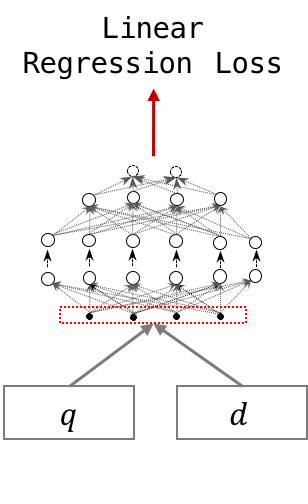
\includegraphics[height=5cm]{03-part-02/chapter-04/figs_and_tables/fig_model_1.png}%
        \caption{\label{fig:m1}\mone model}
    \end{subfigure}%
    ~
    \begin{subfigure}[t]{0.40\columnwidth}
        \centering
        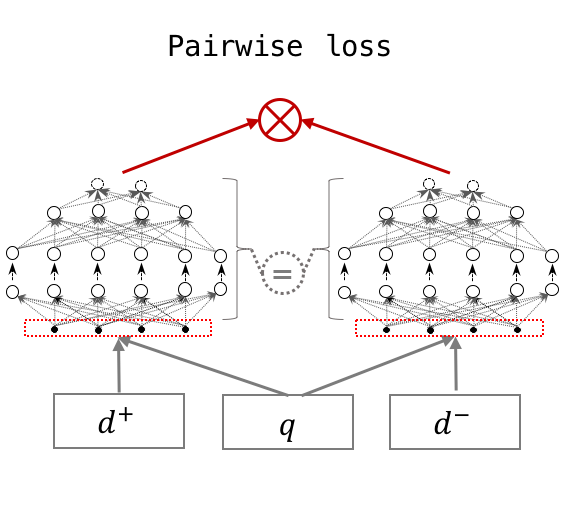
\includegraphics[height=5cm]{03-part-02/chapter-04/figs_and_tables/fig_model_2.png}%
        \caption{\label{fig:m2}\mtwo model}
    \end{subfigure}%
    ~
    \begin{subfigure}[t]{0.37\columnwidth}
        \centering
        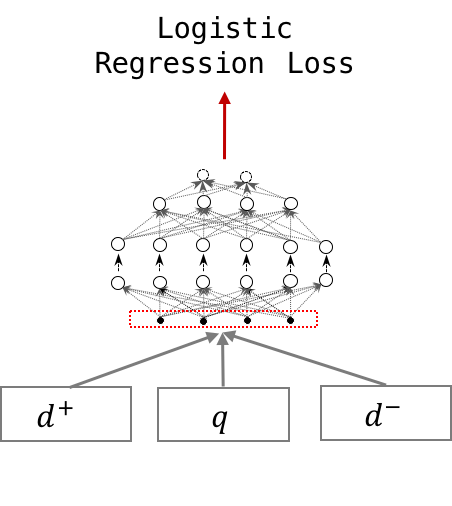
\includegraphics[height=5cm]{03-part-02/chapter-04/figs_and_tables/fig_model_3.png}%
        \caption{\label{fig:m3}\mthree model}
    \end{subfigure}%
    \caption{\label{fig:ranking-arch} Different ranking architectures.}
\end{figure}
%

We define three different ranking models, one point-wise and two pair-wise models:

\subsubsection{\label{sec:modelone}\Modelone}: This architecture models a point-wise ranking model that learns to predict retrieval scores for query-document pairs. More formally, the goal in this architecture is to learn a \emph{scoring function} $\mathcal{S}(q, d; \theta)$ that determines the retrieval score of document $d$ for query $q$, given a set of model parameters $\theta$.
%
In the training stage, we are given a training set comprising of training samples each a triple $x = (q,d, s_{q,d})$, where $q$ is a query from training query set $Q$, $d$ represents a retrieved document for the query $q$, and $s_{q,d}$ is the relevance score (calculated by a weak supervisor), which is acquired using a retrieval scoring function in our setup.
%
We consider the mean squared error as the loss function for a given batch of training samples:
\begin{equation}
\mathcal{L}(b; \theta) = \frac{1}{|b|} \sum_{i=1}^{|b|}{(\mathcal{S}(\{q, d\}_i; \theta) - s_{\{q, d\}_i})^2}
\end{equation}
where $\{q, d\}_i$ denotes the query and the corresponding retrieved document in the $i^{th}$ training sample, i.e., $x_i$ in the batch $b$.
The conceptual architecture of the model is illustrated in Figure~\ref{fig:m1}.


\subsubsection{\label{sec:modeltwo}\Modeltwo}:
In this model, similar to the previous one, the goal is to learn a scoring function $\mathcal{S}(q, d; \theta)$ for a given pair of query $q$ and document $d$ with the set of model parameters $\theta$. 
However, unlike the previous model, we do not aim to learn a calibrated scoring function. 
In this model, as it is depicted in Figure~\ref{fig:m2}, we use a pair-wise scenario during training in which we have two point-wise networks that share parameters and we update their parameters to minimize a pair-wise loss.
In this model, each training sample has five elements: $x = (q,d_1, d_2, s_{q,d_1}, s_{q,d_2})$.
During the inference, we treat the trained model as a point-wise scoring function to score query-document pairs.

We have tried different pair-wise loss functions and empirically found that the model learned based on the hinge loss (max-margin loss function) performs better than the others. 
Hinge loss is a linear loss that penalizes examples that violate the margin constraint. It is widely used in various learning to rank algorithms, such as Ranking SVM~\citep{Herbrich:1999}. The hinge loss function for a batch of training samples is defined as follows:
\begin{equation}
\begin{aligned}
\mathcal{L}(b; \theta) = \frac{1}{|b|}
\sum_{i=1}^{|b|}
\max\big\{
& 
0, \varepsilon - \text{sign}
(s_{\{q, d_1\}_i} - s_{\{q, d_2\}_i})
& \\ & 
\left(\mathcal{S}\left(\{q, d_1\}_i; \theta\right) -\mathcal{S}\left(\{q, d_2\}_i; \theta\right)\right)
\big\}
, 
%\nonumber
\end{aligned}     
\end{equation}
where $\varepsilon$ is the parameter determining the margin of hinge loss. We found that as we compress the outputs to the range of $[-1, 1]$, $\varepsilon=1$ works well as the margin for the hinge loss function.

\subsubsection{\label{sec:modelthree}\Modelthree}:
The third architecture is based on a pair-wise scenario during both training and inference (Figure~\ref{fig:m3}). This model learns a \emph{ranking function} $\mathcal{R}(q, d_1, d_2; \theta)$ which predicts the probability of document $d_1$ to be ranked higher than $d_2$ given $q$.
Similar to the \modeltwo, each training sample has five elements: $x = (q,d_1, d_2, s_{q,d_1}, s_{q,d_1})$.
For a given batch of training samples, we define our loss function based on cross-entropy as follows:
\begin{align}
\mathcal{L}(b; \theta) = -\frac{1}{|b|}
\sum_{i=1}^{|b|} &
P_{\{q,d_1,d_2\}_i} \log(\mathcal{R}(\{q,d_1,d_2\}_i; \theta)) \\
&
+ (1- P_{\{q,d_1,d_2\}_i})\log(1- \mathcal{R}(\{q,d_1,d_2\}_i; \theta)) \nonumber
\end{align}
where $P_{\{q,d_1,d_2\}_i}$ is the probability of document $d_1$ being ranked higher than $d_2$, based on the scores obtained from training sample $x_i$:
\begin{equation}
P_{\{q,d_1,d_2\}_i} = \frac{s_{\{q,d_1\}_i}}{s_{\{q,d_1\}_i} + s_{\{q,d_2\}_i}}
\end{equation}

A similar loss function has been previously used in RankNet~\citep{Burges:2005}. It is notable that at inference time, we need a scalar score for each document. Therefore, we need to turn the model's pair-wise predictions into a score per document. To do so, for each document, we calculate the average of predictions against all other candidate documents, which has $O(n^2)$ time complexity and is not practical in real-world applications. There are some approximations could be applicable to decrease the time complexity at inference time~\citep{Wauthier:2013}.

\medskip
As shown in Figure~\ref{fig:ranking-arch}, all the described ranking architectures share a neural network module. In all these models, we opted for a simple feed-forward neural network which is composed of: input layer $z_0$, $l-1$ hidden layers, and the output layer $z_l$. The input layer $z_0$ provides a mapping $\psi$ to encode the input query and document(s) into a fixed-length vector.
The exact specification of the input representation feature function $\psi$ is given in the next subsection. 
Each hidden layer $z_i$ is a fully-connected layer that computes the following transformation:
\begin{equation}
    z_i = \alpha(W_i.z_{i-1} + b_i); ~ 1<i<l-1,
\end{equation}
where $W_i$ and $b_i$ respectively denote the weight matrix and the bias term corresponding to the $i^{th}$ hidden layer, and $\alpha(.)$ is the activation function. We use the rectifier linear unit $\textit{ReLU}(x) = \max(0, x)$ as the activation function, which is a common choice in the deep learning literature~\citep{Lecun:2015}. 
The output layer $z_l$ is a fully-connected layer with a single continuous output. The activation function for the output layer depends on the ranking architecture that we use. For the \modelone architecture, we empirically found that a linear activation function works best, while $tanh$ and the sigmoid functions are used for the \modeltwo and \modelthree respectively.

Furthermore, to prevent feature co-adaptation, we use dropout as the regularization technique in all the models. Dropout sets a portion of hidden units to zero during the forward phase when computing the activations which prevents overfitting.


\subsection{Representing Inputs}
\label{sec:feedings}
We explore three definitions of the input layer representation $z_0$ captured by a feature function $\psi$ that maps the input into a fixed-size vector which is further fed into the fully connected layers: 
(i) a conventional dense feature vector representation that contains various statistics describing the input query-document pair, 
(ii) a sparse vector containing bag-of-words representation, and 
(iii) bag-of-embeddings averaged with learned weights. 
These input representations define how much capacity is given to the network to extract discriminative signal from the training data and thus result in different generalization behavior of the networks. 
It is noteworthy that input representation of the networks in the \modelone and \modeltwo is defined for a pair of the query and the document, while the network in the \modelthree needs to be fed by a triple of the query, the first document, and the second document.

\subsubsection{\Feedone (\fone)}: 
In this setting, we build a dense feature vector composed of features used by traditional IR methods, e.g., BM25. The goal here is to let the network fit the function described by the BM25 formula when it receives exactly the same inputs. 
In more detail, our input vector is a concatenation ($||$) of the following inputs: total number of documents in the collection (i.e., $N$), average length of documents in the collection (i.e., $avg(l_d)_D$), document length (i.e., $l_d$), frequency of each query term $t_i$ in the document (i.e., $tf(t_i, d)$), and document frequency of each query term (i.e., $df(t_i)$). Therefore, for the point-wise setting, we have the following input vector:
\begin{equation}
\psi(q, d) = [N || avg(l_d)_D || l_d || \{df(t_i) || tf(t_i,d)\}_{1 \leq i \leq k}],
\end{equation}
where $k$ is set to a fixed value ($5$ in our experiments). 
We truncate longer queries and do zero padding for shorter queries. 
For the networks in the \modelthree, we consider a similar function with additional elements: the length of the second document and the frequency of query terms in the second document.


\subsubsection{\Feedtwo (\ftwo)}: 
Next, we move away from a fully featurized representation that contains only aggregated statistics and let the network performs feature extraction for us. In particular, we build a bag-of-words representation by extracting term frequency vectors of query ($tfv_q$), document ($tfv_d$), and the collection ($tfv_c$) and feed the network with concatenation of these three vectors. For the point-wise setting, we have the following input vector:
\begin{equation}
\psi(q, d) = [tfv_c || tfv_q || tfv_d]
\end{equation}
For the network in \modelthree, we have a similar input vector with both $tfv_{d_1}$ and $tfv_{d_2}$. Hence, the size of the input layer is $3 \times vocab~size$ in the point-wise setting, and $4 \times vocab~size$ in the pair-wise setting. 
%In this paradigm, we have no document-level statistic, e.g., document frequency, although collection term frequency would be considered as a clue for term weighting. 

\subsubsection{\label{sec:feedthree}\Feedthree (\fthree)}:
The major weakness of the previous input representation is that words are treated as discrete units, hence prohibiting the network from performing soft matching between semantically similar words in queries and documents. In this input representation paradigm, we rely on word embeddings to obtain more powerful representations of queries and documents that could bridge the lexical chasm. % of \fthree.
The representation function $\psi$ consists of three components: an embedding function $\mathcal{E}: \mathcal{V} \rightarrow \mathbb{R}^{m}$ (where $\mathcal{V}$ denotes the vocabulary set and $m$ is the embedding dimension), a weighting function $\mathcal{W}: \mathcal{V} \rightarrow \mathbb{R}$, and a compositionality function $\odot: (\mathbb{R}^{m}, \mathbb{R})^n \rightarrow \mathbb{R}^{m}$. More formally, the function $\psi$ for the point-wise setting is defined as:
\begin{equation}
\psi(q, d) = [\odot_{i=1}^{|q|}(\mathcal{E}(t_i^q), \mathcal{W}(t_i^q)) || \odot_{i=1}^{|d|} (\mathcal{E}(t_i^d), \mathcal{W}(t_i^d))],
\end{equation}
where $t_i^q$ and $t_i^d$ denote the $i^{th}$ term in query $q$ and document $d$, respectively. 
For the network of the \modelthree, another similar term is concatenated with the above vector for the second document. The embedding function $\mathcal{E}$ transforms each term to a dense $m$-dimensional float vector as its representation, which is learned during the training phase. The weighting function $\mathcal{W}$ assigns a weight to each term in the vocabulary set, which is supposed to learn term global importance for the retrieval task. The compositionality function $\odot$ projects a set of $n$ embedding and weighting pairs to an $m$-dimensional representation, independent from the value of $n$. The compositionality function is given by:
\begin{equation}
\odot_{i=1}^n(\mathcal{E}(t_i), \mathcal{W}(t_i)) = \sum_{i=1}^n \widehat{\mathcal{W}}(t_i)\cdot \mathcal{E}(t_i),
\end{equation}
which is the weighted element-wise sum of the terms' embedding vectors. $\widehat{\mathcal{W}}$ is the normalized weight that is learned for each term, given as follows:
\begin{equation}
\widehat{\mathcal{W}}(t_i) = \frac{\exp(\mathcal{W}(t_i))}{\sum_{j=1}^n{ \exp(\mathcal{W}(t_j))}}
\end{equation}

\medskip
All combinations of different ranking architectures and different input representations presented in this section can be considered for developing ranking models.

\subsection{Training Neural Rankers with Weak Supervision}
In this section,  we discuss the effectiveness of our neural rankers with different learning objectives (Section~\ref{sec:models}) and different input representations (Section~\ref{sec:feedings}), when they are trained with weakly supervised signals.

In the following, we first describe the train and evaluation data, metrics we report, and detailed experimental setup. Then we discuss the results.

% !TEX root = main.tex
\begin{table}
\centering
\caption{Collections statistics.}
\begin{tabularx}{\linewidth}{Xlcrr} 
\toprule
\bf Collection & \bf Genre & \bf Queries & \bf \# docs & \bf length  \\ %\specialcell{avg doc\\length}  \\ 
\midrule
%Robust & news articles & \specialcell{301-450 \\ 601-700} & 528k & 254  \\ %\hline
\bf Robust04 & news  & 301--450,601--700 & 528k & 254  \\ %\hline
\bf ClueWeb & webpages & 1--200 & 50m & 1,506  \\ 
\bottomrule
% GOV2 & \specialcell{2004 crawl of .gov domains} & \specialcell{TREC 2004-2006 Terabyte Track,\\topics 701-850} & 25,205k  & 648 & 26,917  \\ \hline
\end{tabularx}
\label{tab:data}
\end{table}
\subsubsection{Collections}
\label{sec:collections}
In our experiments, we used two standard TREC collections: The first collection (called \emph{Robust04}) consists of over 500k news articles from different news agencies, that is available in TREC Disks 4 and 5 (excluding Congressional Records). This collection, which was used in TREC Robust Track 2004, is considered as a homogeneous collection, because of the nature and the quality of documents. The second collection (called \emph{ClueWeb}) that we used is ClueWeb09 Category B, a large-scale web collection with over 50 million English documents, which is considered as a heterogeneous collection. This collection has been used in TREC Web Track, for several years. In our experiments with this collection, we filtered out the spam documents using the Waterloo spam scorer\footnote{\url{http://plg.uwaterloo.ca/~gvcormac/clueweb09spam/}}~\citep{Cormack:2011} with the default threshold $70\%$. The statistics of these collections are reported in Table~\ref{tab:data}. 

\subsubsection{Training query set}
\label{sec:query_set}
To train our neural ranking models, we used the unique queries (only the query string) appearing in the AOL query logs~\citep{Pass:2006}. This query set contains web queries initiated by real users in the AOL search engine that were sampled from a three-month period from March 1, 2006 to May 31, 2006. We filtered out a large volume of navigational queries containing URL substrings (``http'', ``www.'', ``.com'', ``.net'', ``.org'', ``.edu''). We also removed all non-alphanumeric characters from the queries. We made sure that no queries from the training set appear in our evaluation sets. For each dataset, we took queries that have at least ten hits in the target corpus using the pseudo-labeler method. Applying all these processes, we ended up with 6.15 million queries for the Robust04 dataset and 6.87 million queries for the ClueWeb dataset. 
In our experiments, we randomly selected $80\%$ of the training queries as training set and the remaining $20\%$ of the queries were chosen as the validation set for hyper-parameter tuning. As the ``pseudo-labeler'' in our training data, we have used BM25 to score/rank documents in the collections given the queries in the training query set.

\subsubsection{Evaluation query sets} 
We use the following query sets for evaluation that contain human-labeled judgments: a set of 250 queries (TREC topics 301--450 and 601--700) for the Robust04 collection that were previously used in TREC Robust Track 2004. A set of 200 queries (topics 1-200) were used for the experiments on the ClueWeb collection. These queries were used in TREC Web Track 2009--2012. We only used the title of topics as queries.

\subsubsection{Evaluation Metrics}
To evaluate retrieval effectiveness, we report three standard evaluation metrics: mean average precision (MAP) of the top-ranked $1000$ documents, precision of the top $20$ retrieved documents (P@20), and normalized discounted cumulative gain (nDCG)~\citep{Jarvelin:2002} calculated for the top $20$ retrieved documents (nDCG@20). Statistically significant differences of MAP, P@20, and nDCG@20 values are determined using the two-tailed paired t-test with $p\_value<0.05$, with Bonferroni correction.


\subsubsection{Experimental Setup}
All models described in Section~\ref{sec:models} are implemented using TensorFlow~\citep{tang2016:tflearn,tensorflow2015-whitepaper}.
In all experiments, the parameters of the network are optimized employing the Adam optimizer~\citep{Kingma:2014} and using the computed gradient of the loss to perform the back-propagation algorithm.
All model hyper-parameters were tuned on the respective validation set using batched GP bandits with an expected improvement acquisition function~\citep{Desautels:2014}. 
For each model, the size of hidden layers and the number of hidden layers were selected from $[16, 32, 64, 128, 256, 512, 1024]$ and $[1, 2, 3, 4]$, respectively. The initial learning rate and the dropout parameter were selected from $[1E-3, 5E-4, 1E-4, 5E-5, 1E-5]$ and $[0.0, 0.1, 0.2, 0.5]$, respectively. For models with \feedthree, we considered embedding sizes of $[100, 300, 500, 1000]$. As the training data, we take the top $1000$ retrieved documents for each query from training query set $Q$, to prepare the training data. In total, we have $|Q|\times 1000$ ($\sim6E10$ examples in our data) point-wise example and $\sim|Q|\times 1000^2$ ($\sim6E13$ examples in our data) pair-wise examples. The batch size in our experiments was selected from  $[128, 256, 512]$.
%
At inference time, for each query, we take the top $2000$ retrieved documents using BM25 as candidate documents and re-rank them by the trained models. In our experiments, we use the Indri\footnote{\url{https://www.lemurproject.org/indri.php}} implementation of BM25 with the default parameters (i.e., $k_1 = 1.2$, $b = 0.75$, and $k_3 = 1000$).


\bigskip
Given the setup we explained above, we train and evaluate our neural rankers to address our second research question in this chapter:
\resq{c4.2}

We attempt to break down our experiments and analyses to different parts addressing several subquestions, and provide empirical answers along with the intuition and analysis behind each question:

% !TEX root = main.tex
\begin{table*}[tbp]
\centering
\caption{\label{tbl_main}Performance of the different models on different datasets. \ps or \ns indicates that the improvements or degradations with respect to BM25 are statistically significant, at the 0.05 level using the paired two-tailed t-test.}
%\begin{adjustbox}{max width=\columnwidth}
%\begin{tabular}{@{}l@{~~~}c@{~~}c@{~~}c@{~~~}c@{~~}c@{~~}c@{}}
\begin{adjustbox}{max width=\textwidth}
\begin{tabular}{l c c c c c c}
\toprule
\multirow{2}{*}{\textbf{Method}} &
%\multicolumn{1}{l}{\textbf{Method}} & 
\multicolumn{3}{c}{\textbf{Robust04}} & \multicolumn{3}{c}{\textbf{ClueWeb}}
\\ \cmidrule(lr){2-4} \cmidrule(lr){5-7}
& \textit{MAP} & \textit{P@20} & \textit{nDCG@20}  & \textit{MAP} & \textit{P@20} & \textit{nDCG@20}
\\ \midrule
\textbf{BM25} 
& 0.2503\fs & 0.3569\fs & 0.4102\fs  
& 0.1021\fs & 0.2418\fs & 0.2070\fs
\\ \midrule
\textbf{\mone + \fone} 
& 0.1961\ns & 0.2787\ns & 0.3260\ns 
& 0.0689\ns & 0.1518\ns & 0.1430\ns
\\ 
\textbf{\mone + \ftwo} 
& 0.2141\ns & 0.3180\ns & 0.3604\ns 
& 0.0701\ns & 0.1889\ns & 0.1495\ns
\\ 
\textbf{\mone + \fthree} 
& 0.2423\ns & 0.3501\fs & 0.3999\fs 
& 0.1002\fs & 0.2513\fs & 0.2130\fs
\\ \midrule
\textbf{\mtwo + \fone} 
& 0.1940\ns & 0.2830\ns & 0.3317\ns 
& 0.0622\ns & 0.1516\ns & 0.1383\ns
\\ 
\textbf{\mtwo + \ftwo} 
& 0.2213\ns & 0.3216\ns & 0.3628\ns 
& 0.0776\ns & 0.1989\ns & 0.1816\ns
\\ 
\textbf{\mtwo + \fthree} 
& \textbf{0.2811}\ps & \textbf{0.3773}\ps & \textbf{0.4302}\ps 
& \textbf{0.1306}\ps & \textbf{0.2839}\ps & \textbf{0.2216}\ps
\\ \midrule
\textbf{\mthree + \fone} 
& 0.2192\ns & 0.2966\ns & 0.3278\ns 
& 0.0702\ns & 0.1711\ns & 0.1506\ns
\\ 
\textbf{\mthree + \ftwo} 
& 0.2246\ns & 0.3250\ns & 0.3763\ns 
& 0.0894\ns & 0.2109\ns & 0.1916\fs
\\ 
\textbf{\mthree + \fthree} 
& \textbf{0.2837}\ps & \textbf{0.3802}\ps & \textbf{0.4389}\ps 
& \textbf{0.1387}\ps & \textbf{0.2967}\ps & \textbf{0.2330}\ps
\\ \bottomrule
\end{tabular}
\end{adjustbox}
\end{table*} 
\subsubsection{How do the neural models with different training objectives and input representations compare?}
%
Table~\ref{tbl_main} presents the performance of all model combinations.
Interestingly, combinations of the \modeltwo and the \modelthree with \feedthree outperform BM25 by significant margins in both collections. For instance, the \modelthree with \feedthree that shows the best performance among the other methods, surprisingly, improves BM25 by over $13\%$ and $35\%$ in Robust04 and ClueWeb collections respectively, in terms of MAP. Similar improvements can be observed for the other evaluation metrics.

Regarding the modeling architecture, in the \modeltwo and the \modelthree, compared to the \modelone, we define objective functions that target to learn ranking instead of scoring. This is particularly important in weak supervision, as the scores are imperfect values---using the ranking objective alleviates this issue by forcing the model to learn a preference function rather than reproduce absolute scores.
%
In other words, using the ranking objective instead of learning to predict calibrated scores allows the \modeltwo and the \modelthree to learn to distinguish between examples whose scores are close. This way, some small amount of noise, which is a common problem in weak supervision, would not perturb the ranking as easily~\citep{Zamani:2018:ictir}.

Regarding the input representations, \feedthree leads to better performance compared to the other ones in all models.
Using \feedthree not only provides the network with more information, but also lets the network to learn proper representation capturing the needed elements for the next layers with a better understanding of the interactions between query and documents. 
Providing the network with already engineered features would block it from going beyond the weak supervision signal and limit the ability of the models to learn latent features that are unattainable through feature engineering. 

Note that although the \modelthree is more precise in terms of MAP, the \modeltwo is much faster in the inference time ($O(n)$ compared to $O(n^2)$), which is a desirable property in real-life applications.

% !TEX root = main.tex
\begin{figure*}[t]
    \centering
    \begin{subfigure}[t]{0.33\textwidth}
        \centering
        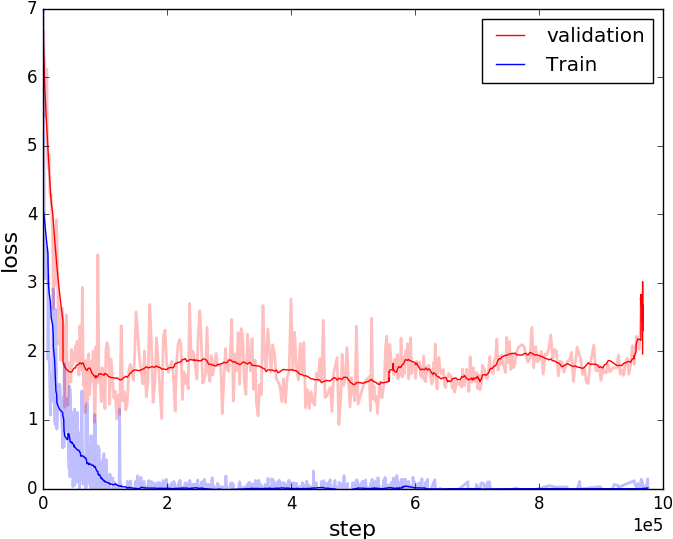
\includegraphics[height=3.6cm]{03-part-02/chapter-04/figs_and_tables/loss_step_plots/step_m1f1.png}
        \caption{\label{fig:m1f1}\mone-\fone}
    \end{subfigure}%
    ~
    \begin{subfigure}[t]{0.33\textwidth}
        \centering
        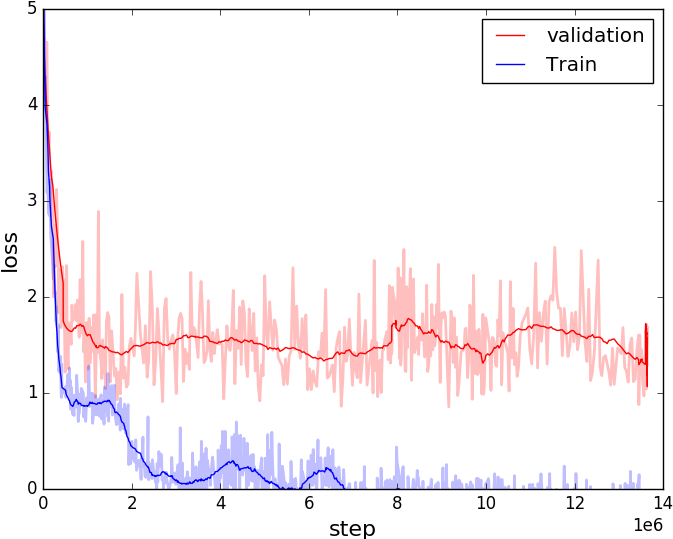
\includegraphics[height=3.6cm]{03-part-02/chapter-04/figs_and_tables/loss_step_plots/step_m1f2.png}
        \caption{\label{fig:m1f2}\mone-\ftwo}
    \end{subfigure}%
    ~
    \begin{subfigure}[t]{0.33\textwidth}
        \centering
        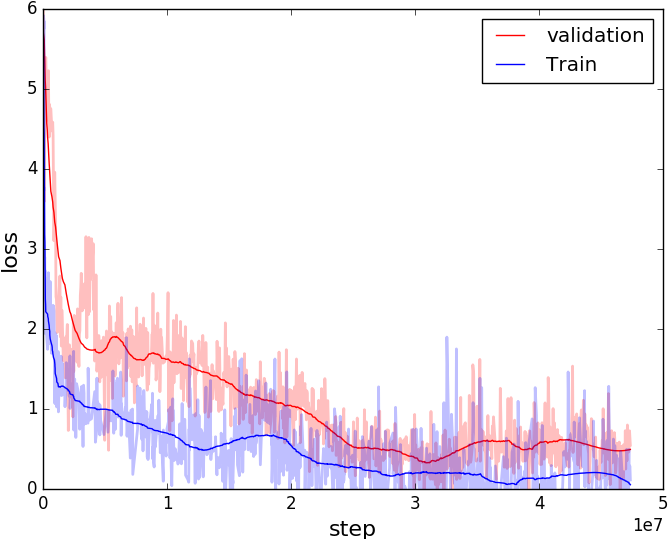
\includegraphics[height=3.6cm]{03-part-02/chapter-04/figs_and_tables/loss_step_plots/step_m1f3.png}
        \caption{\label{fig:m1f3}\mone-\fthree}
    \end{subfigure}%
    \\
    \begin{subfigure}[t]{0.33\textwidth}
        \centering
        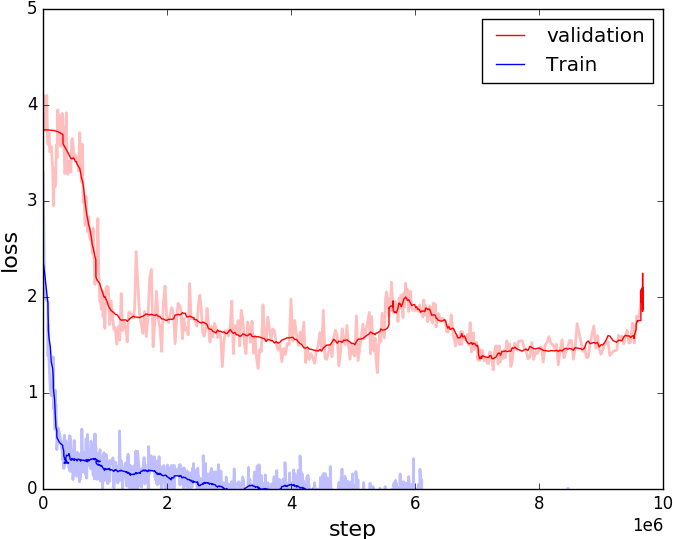
\includegraphics[height=3.6cm]{03-part-02/chapter-04/figs_and_tables/loss_step_plots/step_m2f1.png}
        \caption{\label{fig:m2f1}\mtwo-\fone}
    \end{subfigure}%
    ~
    \begin{subfigure}[t]{0.33\textwidth}
        \centering
        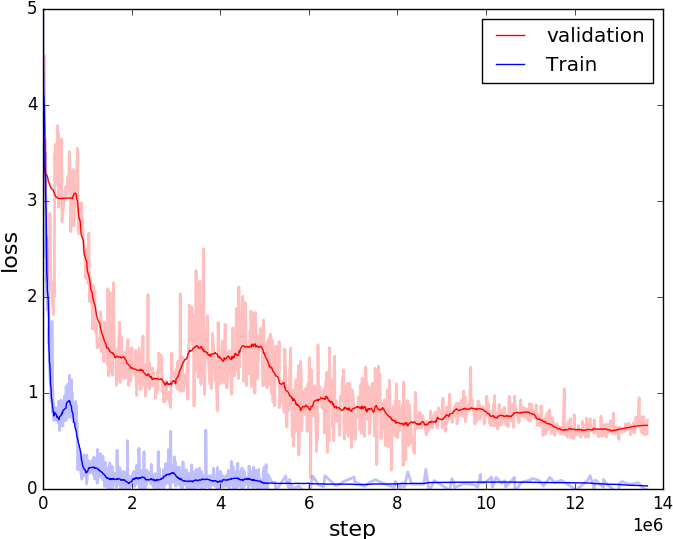
\includegraphics[height=3.6cm]{03-part-02/chapter-04/figs_and_tables/loss_step_plots/step_m2f2.png}
        \caption{\label{fig:m2f2}\mtwo-\ftwo}
    \end{subfigure}%
    ~
    \begin{subfigure}[t]{0.33\textwidth}
        \centering
        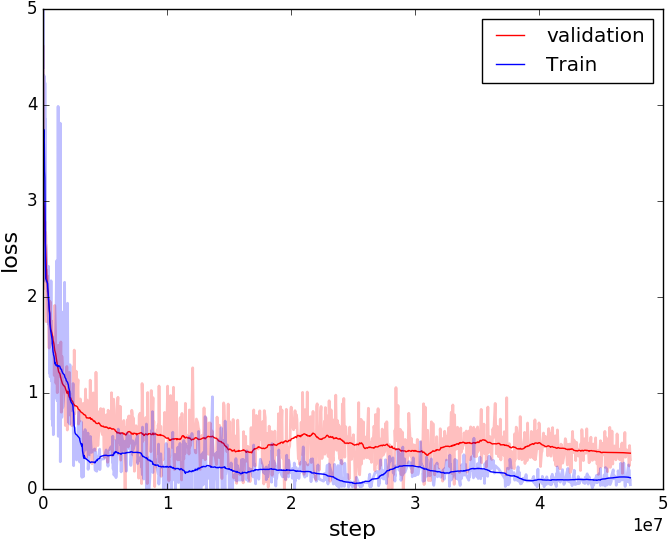
\includegraphics[height=3.6cm]{03-part-02/chapter-04/figs_and_tables/loss_step_plots/step_m2f3.png}
        \caption{\label{fig:m2f3}\mtwo-\fthree}
    \end{subfigure}%
        \\
    \begin{subfigure}[t]{0.33\textwidth}
        \centering
        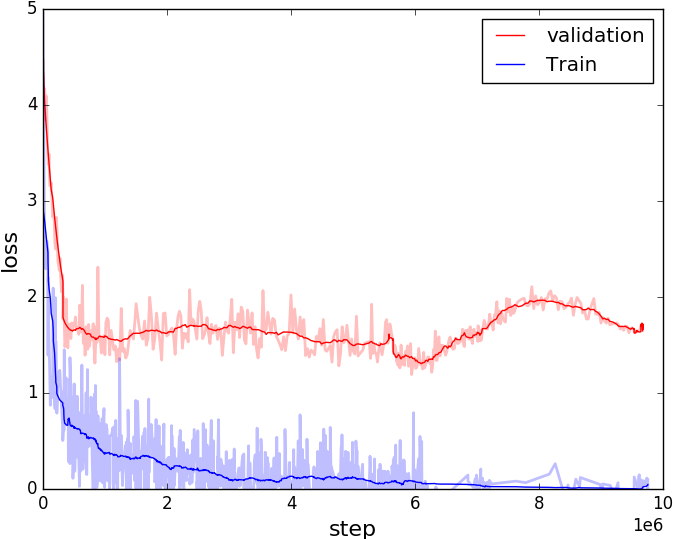
\includegraphics[height=3.6cm]{03-part-02/chapter-04/figs_and_tables/loss_step_plots/step_m3f1.png}
        \caption{\label{fig:m3f1}\mthree-\fone}
    \end{subfigure}%
    ~
    \begin{subfigure}[t]{0.33\textwidth}
        \centering
        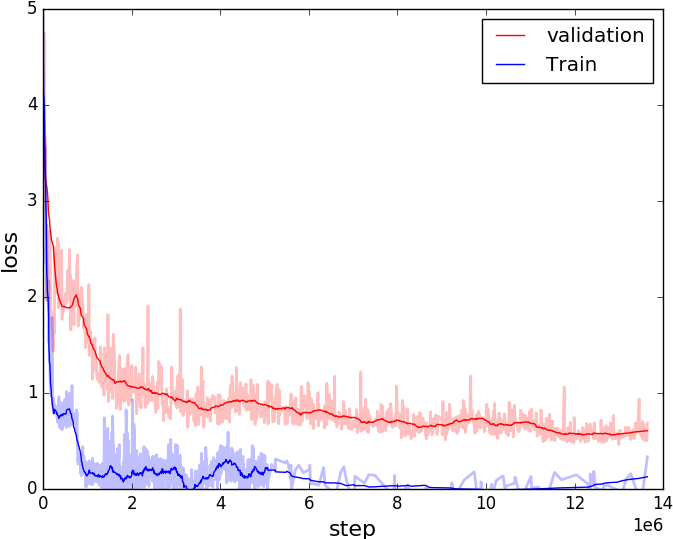
\includegraphics[height=3.6cm]{03-part-02/chapter-04/figs_and_tables/loss_step_plots/step_m3f2.png}
        \caption{\label{fig:m3f2}\mthree-\ftwo}
    \end{subfigure}%
    ~
    \begin{subfigure}[t]{0.33\textwidth}
        \centering
        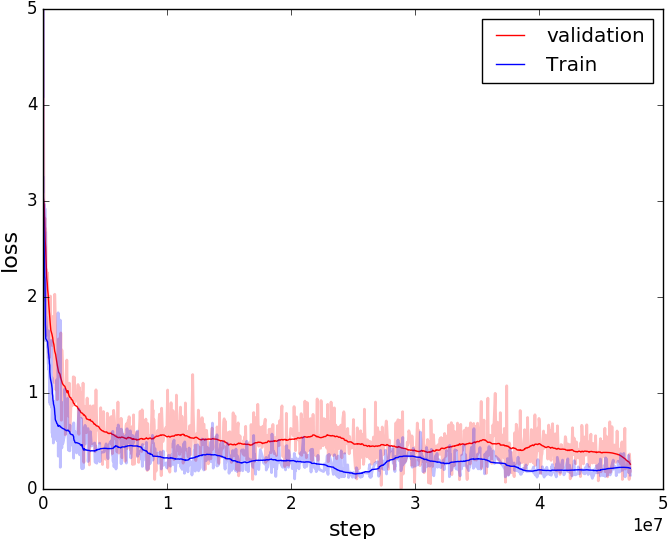
\includegraphics[height=3.6cm]{03-part-02/chapter-04/figs_and_tables/loss_step_plots/step_m3f3.png}
        \caption{\label{fig:m3f3}\mthree-\fthree}
    \end{subfigure}%
    \caption{Training and validation loss curves for all combinations of different ranking architectures and feeding paradigms.}
    \label{fig:step-loss}
\end{figure*}

\subsubsection{Why do \feedone and \feedtwo fail to replicate the performance of BM25?}
%
Although neural networks are capable of approximating arbitrarily complex non-linear functions, we observe that the models with \feedone fail to replicate the BM25 performance, while they are given the same feature inputs as the BM25 components (e.g., TF, IDF, average document length, etc). To ensure that the training converges and there is no overfitting, we have looked into the training and validation loss values of different models during the training time. Figure~\ref{fig:step-loss} illustrates the loss curves for the training and validation sets per training step for different models.
%
As shown, in models with \feedone, the training losses drop quickly to values close to zero while this is not the case for the validation losses, which is an indicator of over-fitting on the training data. 
Although we have tried different regularization techniques, like $l_2$-regularization and dropout with various parameters, there is less chance for generalization when the networks are fed with the fully featurized input. Note that over-fitting would lead to poor performance, especially in weak supervision scenarios as the network learns to model imperfections from weak annotations. 
%
This phenomenon is also the case for models with the \feedtwo, but with less impact. However, in the models with the \feedthree, the networks do not overfit, which helps it to go beyond the weak supervision signals in the training data.

\begin{figure}[!t]
\pgfplotsset{ticks=none}
\centering
\begin{tikzpicture}
\begin{axis}[
        width= 14cm, 
        height=8cm,
        grid = both,
        nodes near coords, %={(\coordindex)},
        scatter/classes={
        	BM25={mark=otimes*, mark size=3pt, yellow, draw = black},%
        	m1f1={mark=halfcircle*, mark size=3pt, blue, },%
        	m1f2={mark=halfcircle*, mark size=3pt, red},%
        	m1f3={mark=halfcircle*, mark size=3pt, black},
        	m2f1={mark=halfsquare*, mark size=3pt, blue},%
        	m2f2={mark=halfsquare*, mark size=3pt, red},%
        	m2f3={mark=halfsquare*, mark size=3pt, black},
        	m3f1={mark=pentagon*, mark size=3pt, blue},%
        	m3f2={mark=pentagon*, mark size=3pt, red},%
        	m3f3={mark=pentagon*, mark size=3pt, black}
    	},
    	legend style={
            % legend image post style={xscale=0.75},
            % inner sep=0pt,
            at={(1.2,0.85)},
            % anchor=west,
            font=\fontsize{6}{7}\selectfont,
        },
    	]
	\addplot[scatter,only marks,
		scatter src=explicit symbolic]
		coordinates {
			(0.403,0.801) [BM25]
			(0.341,0.749) [m1f1]
			(0.232,0.240) [m1f2]
			(0.570,0.412) [m1f3]
			(0.091,0.718) [m2f1]
			(0.265,0.369) [m2f2]
			(0.808,0.101) [m2f3]
			(0.246,0.601) [m3f1]
			(0.371,0.600) [m3f2]
			(0.730,0.305) [m3f3]
		};
	\node [right] at (0.413,0.801){\footnotesize{BM25}};
	\node [left] at (0.381,0.800){\footnotesize{\mone + \fone}};
	\node [below] at (0.232,0.230){\footnotesize{\mone + \ftwo}};
	\node [above] at (0.570,0.422){\footnotesize{\mone + \fthree}};
	\node [below] at (0.121,0.708){\footnotesize{\mtwo + \fone}};
	\node [above] at (0.265,0.379){\footnotesize{\mtwo + \ftwo}};
	\node [above] at (0.758,0.121){\footnotesize{\mtwo + \fthree}};
	\node [below] at (0.226,0.591){\footnotesize{\mthree + \fone}};
	\node [right] at (0.381,0.600){\footnotesize{\mthree + \ftwo}};
	\node [above] at (0.730,0.315){\footnotesize{\mthree + \fthree}};
%  	\legend{BM25,m1f1,m1f2,m1f3,m2f1,m2f2,m2f3,m3f1,m3f2,m3f3}
\end{axis}
\end{tikzpicture}
\caption{Proximity of different models in terms of query-by-query performance.
 \label{fig:modelproximity}}
 \end{figure}
\subsubsection{How are the models related?}
%
To better understand the relationship of different neural models described above, we compare their performance across the query dimension following the approach in~\citep{Mitra:2016}. 
We assume that similar models should perform similarly for the same queries. Hence, we represent each model by a vector, called the performance vector, whose elements correspond to per query performance of the model, in terms of nDCG@20. The closer the performance vectors are, the more similar the models are in terms of the query by query performance. For the sake of visualization, we reduce the vectors dimension by projecting them to a two-dimensional space, using t-Distributed Stochastic Neighbor Embedding (t-SNE)\footnote{\url{https://lvdmaaten.github.io/tsne/}}.

Figure~\ref{fig:modelproximity} illustrates the proximity of different models in the Robust04 collection. Based on this plot, models with similar input representations (same color) have quite close performance vectors, which means that they perform similarly for the same queries. This is not necessarily the case for models with similar architecture (same shape). 
This suggests that the amount and the way that we provide information to the networks are the key factors in the ranking performance. 

We also observe that the \modelone with \feedone is the closest to BM25 which is expected. 
It is also interesting that models with \feedthree are placed far away from other models which shows they perform differently compared to the other input representations.


\subsubsection{How meaningful are the compositionality weights learned in the \feedthree?}
%
In this experiment, we focus on the best performing combination, i.e., the \modelthree with \feedthree. To analyze what the network learns, we look into the weights $\mathcal{W}$ (see Section~\ref{sec:feedthree}) learned by the network. Note that the weighting function $\mathcal{W}$ learns a global weight for each vocabulary term. We notice that in both collections there is a strong linear correlation between the learned weights and the inverse document
%
\begin{figure}[!t]%
    \centering
    \begin{subfigure}[t]{0.45\textwidth}
        \centering
        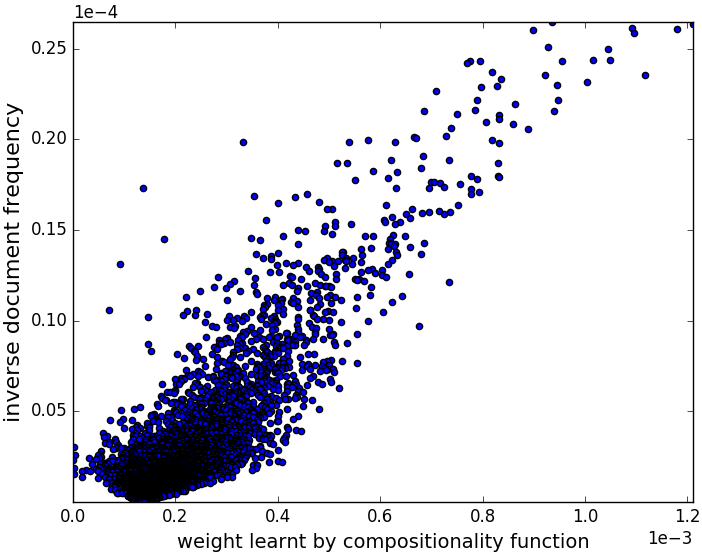
\includegraphics[height=5cm]{03-part-02/chapter-04/figs_and_tables/plot_composionality_idf_scatter_robust.png}
        \caption{\label{fig:scatter_r}Robust04}{\scriptsize{(Pearson Correlation: 0.8243)}}
    \end{subfigure}%
    ~
    \begin{subfigure}[t]{0.45\textwidth}
        \centering
        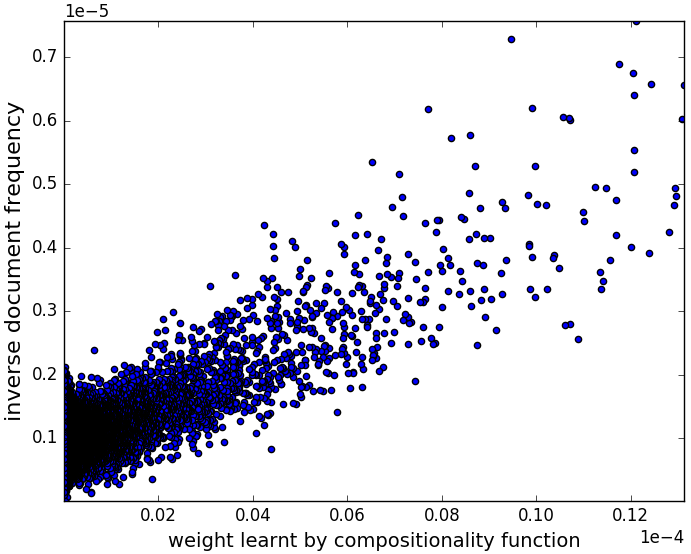
\includegraphics[height=5cm]{03-part-02/chapter-04/figs_and_tables/plot_composionality_idf_scatter_clueweb.png}
        \caption{\label{fig:scatter_c}ClueWeb}{\scriptsize{(Pearson Correlation: 0.7014)}}
    \end{subfigure}%
    \caption{\label{fig:scatter}Strong linear correlation between weight learned by the compositionality function in the \feedthree and inverse document frequency.}
\end{figure}
%
Figure~\ref{fig:scatter} illustrates the scatter plots of the learned weight for each vocabulary term and its IDF, in both collections.
This is an interesting observation as we do not provide any global corpus information to the network in training and the network is able to infer such global information by only observing individual training samples.
% This demonstrates the ability of neural networks to automatically extract meaningful features for the task.

% !TEX root = main.tex
\begin{table*}[tbp]
\centering
\caption{\label{tbl_res_m3f3_em}Performance of the \modelthree with variants of the \feedthree on different datasets. \ps indicates that the improvements over all other models are statistically significant, at the 0.05 level using the paired two-tailed t-test, with Bonferroni correction.}
%\begin{adjustbox}{max width=\columnwidth}
%\begin{tabular}{@{}l@{~~~}c@{~~}c@{~~}c@{~~~}c@{~~}c@{~~}c@{}}
\begin{adjustbox}{max width=\textwidth}
\begin{tabular}{l c c c c c c}
\toprule
\multirow{2}{*}{\textbf{Embedding type}} &
%\multicolumn{1}{l}{\textbf{Method}} & 
\multicolumn{3}{c}{\textbf{Robust04}} & \multicolumn{3}{c}{\textbf{ClueWeb}}
\\ \cmidrule(lr){2-4} \cmidrule(lr){5-7}
& \textit{MAP} & \textit{P@20} & \textit{nDCG@20}  & \textit{MAP} & \textit{P@20} & \textit{nDCG@20}
\\ \midrule
\textbf{Pretrained (external) + Uniform weighting} 
& 0.1656 & 0.2543 & 0.3017 
& 0.0612 & 0.1300 & 0.1401
\\ 
\textbf{Pretrained (external) + IDF weighting} 
& 0.1711 & 0.2755 & 0.3104 
& 0.0712 & 0.1346 & 0.1469
\\ 
\textbf{Pretrained (external) + Weight learning} 
& 0.1880 & 0.2890 & 0.3413 
& 0.0756 & 0.1344 & 0.1583
\\ 
\textbf{Pretrained (target) + Uniform weighting} 
& 0.1217 & 0.2009 & 0.2791 
& 0.0679 & 0.1331 & 0.1587
\\ 
\textbf{Pretrained (target) + IDF weighting} 
& 0.1402 & 0.2230 & 0.2876 
& 0.0779 & 0.1674 & 0.1540
\\ 
\textbf{Pretrained (target) + Weight learning} 
& 0.1477 & 0.2266 & 0.2804 
& 0.0816 & 0.1729 & 0.1608
\\
\textbf{Learned + Uniform weighting} 
& 0.2612 & 0.3602 & 0.4180 
& 0.0912 & 0.2216 & 0.1841
\\
\textbf{Learned + IDF weighting} 
& 0.2676 & 0.3619 & 0.4200 
& 0.1032 & 0.2419 & 0.1922
\\ 
\textbf{Learned + Weight learning} 
& \textbf{0.2837}\ps & \textbf{0.3802}\ps & \textbf{0.4389}\ps
& \textbf{0.1387}\ps & \textbf{0.2967}\ps & \textbf{0.2330}\ps
\\ \bottomrule
\end{tabular}
\end{adjustbox}
\end{table*}

\subsubsection{How well do other alternatives for the embedding and weighting functions in the \feedthree perform?}
Considering \feedthree as the input representation, we have examined different alternatives for the embedding function $\mathcal{E}$: (1) employing pre-trained word embeddings learned from an external corpus (we used Google News), (2) employing pre-trained word embeddings learned from the target corpus (using the skip-gram model \cite{Mikolov:2013}), and (3) learning embeddings during the network training as it is explained in Section~\ref{sec:feedthree}. 
Furthermore, for the compositionality function $\odot$, we tried different alternatives: (1) uniform weighting (simple averaging which is a common approach in compositionality function), (2) using IDF as fixed weights instead of learning the weighting function $\mathcal{W}$, and (3) learning weights during the training as described in Section~\ref{sec:feedthree}.

Table~\ref{tbl_res_m3f3_em} presents the performance of all these combinations on both collections. 
We note that learning both embedding and weighting functions leads to the highest performance in both collections. These improvements are statistically significant.
%
According to the results, regardless of the weighting approach, learning embeddings during training outperforms the models with fixed pre-trained embeddings.
%
This supports the hypothesis that with the \feedthree the neural networks learn an embedding that is based on the interactions of query and documents that tends to be tuned better to the corresponding ranking task.
%
Also, regardless of the embedding method, learning weights helps models to get better performance compared to the fixed weightings, with either IDF or uniform weights. 
%
Although weight learning can significantly affect the performance, it has less impact than learning embeddings.

Note that in the models with pre-trained word embeddings, employing word embeddings trained on the target collection outperforms those trained on the external corpus in the ClueWeb collection; while this is not the case for the Robust04 collection. The reason could be related to the collection size, since the ClueWeb is approximately $100$ times larger than the Robust04.

\begin{figure}[t]
    \centering
    \begin{subfigure}[t]{0.45\textwidth}
        \centering
        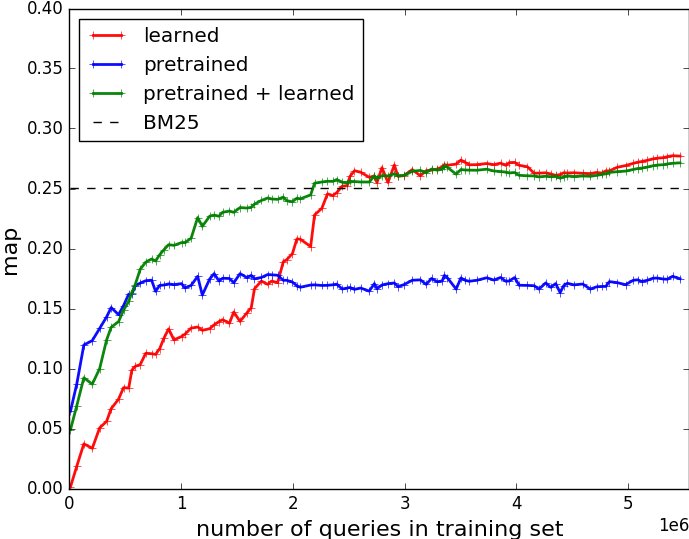
\includegraphics[height=5cm]{03-part-02/chapter-04/figs_and_tables/plot_with_pretrained_emb_robust.png}
        \caption{\label{fig:embedding_r}Robust04}
    \end{subfigure}%
    ~
    \begin{subfigure}[t]{0.45\textwidth}
        \centering
        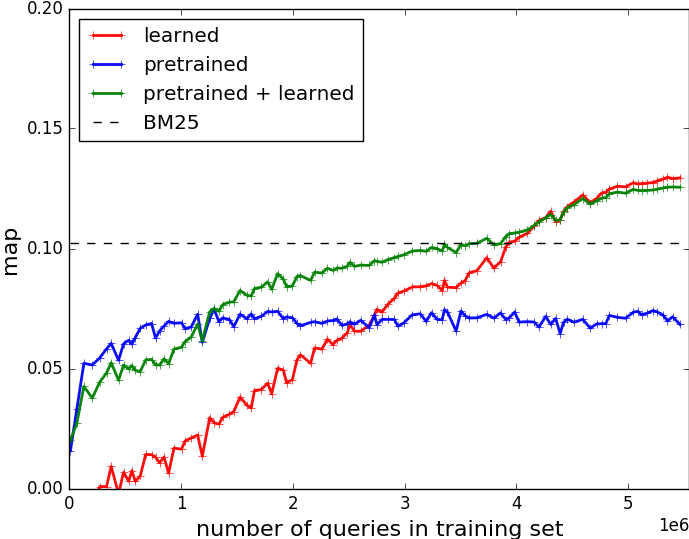
\includegraphics[height=5cm]{03-part-02/chapter-04/figs_and_tables/plot_with_pretrained_emb_clueweb.png}
        \caption{\label{fig:embedding_c}ClueWeb}
    \end{subfigure}%
    \caption{\label{fig:embedding}Performance of the \modelthree with learned embedding, pre-trained embedding, and learned embedding with pre-trained embedding as initialization, with respect to different amount of training data.}
\end{figure}

In addition to the aforementioned experiments, we have also tried initializing the embedding matrix with a pre-trained word embedding trained on the Google News corpus, instead of random initialization.
%
Figure~\ref{fig:embedding} presents the learning curve of the models. According to this figure, the model initialized by a pre-trained embedding performs better than random initialization when a limited amount of training data is available. 
%
When enough training data is fed to the network, initializing with pre-trained embedding and random values converge to the same performance.
An interesting observation here is that in both collections, these two initializations converge when the models exceed the performance of the weak supervision source, which is BM25 in our experiments. 
This suggests that the convergence occurs when accurate representations are learned by the networks, regardless of the initialization.

%In other words, after the network sees enough amount of train data to go beyond the supervision signal, it does not matter that with which initialization the model has started to train.
% !TEX root = main.tex
\begin{table*}[tbp]
\centering
\caption{\label{tbl_svm}Performance of the linear RankSVM with different features.}
%\begin{adjustbox}{max width=\columnwidth}
%\begin{tabular}{@{}l@{~~~}c@{~~}c@{~~}c@{~~~}c@{~~}c@{~~}c@{}}
\begin{adjustbox}{max width=\textwidth}
\begin{tabular}{l c c c c c c}
\toprule
\multirow{2}{*}{\textbf{Method}} &
%\multicolumn{1}{l}{\textbf{Method}} & 
\multicolumn{3}{c}{\textbf{Robust04}} & \multicolumn{3}{c}{\textbf{ClueWeb}}
\\ \cmidrule(lr){2-4} \cmidrule(lr){5-7}
& \textit{MAP} & \textit{P@20} & \textit{nDCG@20}  & \textit{MAP} & \textit{P@20} & \textit{nDCG@20}
\\ \midrule
\textbf{RankSVM + \fone} 
& 0.1983\fs & 0.2841\fs & 0.3375\fs 
& 0.0761\fs & 0.1840\fs & 0.1637\fs
\\ 
\textbf{RankSVM + \ftwo} 
& 0.2307\fs & 0.3260\fs & 0.3794\fs 
& 0.0862\fs & 0.2170\fs & 0.1939\fs
\\ 
\textbf{RankSVM + (Pretrained (external) + IDF weighting)} 
& 0.1539\fs & 0.2121\fs & 0.1852\fs 
& 0.0633\fs & 0.1572\fs & 0.1494\fs 
\\ \midrule
\textbf{\mone (one layer with no nonlinearity) + \fthree} 
& 0.2103\fs & 0.3986\fs & 0.3160\fs 
& 0.0645\fs & 0.1421\fs & 0.1322\fs
\\ \bottomrule
\end{tabular}
\end{adjustbox}
\end{table*}
\subsubsection{Are deep neural networks a good choice for learning to rank with weak supervision?}
%
To see if there is a real benefit from using a non-linear neural network in different settings, we examined RankSVM~\citep{Joachims:2002} as a strong-performing pair-wise learning to rank method with the linear kernel that is fed with different inputs: \feedone, \feedtwo, and \feedthree. Considering that off-the-shelf RankSVM is not able to learn embedding representations during training, for \feedthree, instead of learning embeddings we use a pre-trained embedding matrix trained on Google News and fixed IDF weights. 

The results are reported in Table~\ref{tbl_svm}. As BM25 is not a linear function, RankSVM with the linear kernel is not able to completely approximate it. However, surprisingly, for both \feedone and \feedtwo, RankSVM works as well as neural networks (see Table~\ref{tbl_main}). 
%
Also, compared to the corresponding experiment in Table~\ref{tbl_res_m3f3_em}, the performance of the neural network with an external pre-trained embedding and IDF weighting is not considerably better than RankSVM. 
This shows that having non-linearity in neural networks does not help that much when we do not have representation learning as part of the model.
%
Note that all of these results are still lower than BM25, which shows that they are not good at learning from weak supervision signals for ranking. 
%

We have also examined the \modelone with a network with a single linear hidden layer, with the \feedthree, which is equivalent to a linear regression model with the ability of representation learning. 
Comparing the results of this experiment with \mone-\fthree in Table~\ref{tbl_main}, we can see that with a single-linear network we are not able to achieve a performance that is as good as a deep neural network with non-linearity.
%
This shows that the most important superiority of deep neural networks over other machine learning methods is their ability to learn an effective representation and take all the interactions between query and document(s) into consideration for approximating an effective ranking/scoring function. 
This can be achieved when we have a deep enough network with non-linear activations.

%\alexi{Mosi@: we should also include supervised learning experiments on smaller subsets of human judgments, if possible. The idea is that in these scenarios where labeled data is scarce, weak supervision is really useful. Having plots, where we use various percentages of labeled examples and observing how weak supervision is increasingly important as the number of labeled examples becomes smaller.}
% !TEX root = main.tex
\begin{table*}[tbp]
\centering
\caption{Performance of the \modelthree with \feedthree in fully supervised setting, weak supervised setting, and weak supervised plus supervision as fine tuning. \ps indicates that the improvements over all other models are statistically significant, at the 0.05 level using the paired two-tailed t-test, with Bonferroni correction.}
\label{tbl_semisup}
%\begin{adjustbox}{max width=\columnwidth}
%\begin{tabular}{@{}l@{~~~}c@{~~}c@{~~}c@{~~~}c@{~~}c@{~~}c@{}}
\begin{adjustbox}{max width=\textwidth}
\begin{tabular}{l c c c c c c}
\toprule
\multirow{2}{*}{\textbf{Method}} &
%\multicolumn{1}{l}{\textbf{Method}} & 
\multicolumn{3}{c}{\textbf{Robust04}} & \multicolumn{3}{c}{\textbf{ClueWeb}}
\\ \cmidrule(lr){2-4} \cmidrule(lr){5-7}
& \textit{MAP} & \textit{P@20} & \textit{nDCG@20}  & \textit{MAP} & \textit{P@20} & \textit{nDCG@20}
\\ \midrule
\textbf{Weakly supervised} 
& 0.2837 \fs & 0.3802\fs & 0.4389\fs  
& 0.1387 \fs & 0.2967\fs & 0.2330\fs
\\
\textbf{Fully supervised} 
& 0.1790 \fs & 0.2863\fs & 0.3402\fs  
& 0.0680 \fs & 0.1425\fs & 0.1652\fs
\\
\textbf{Weakly supervised + Fully supervised} 
& \textbf{0.2912}\ps & \textbf{0.4126}\ps & \textbf{0.4509}\ps 
& \textbf{0.1520}\ps & \textbf{0.3077}\ps & \textbf{0.2461}\ps
\\ \bottomrule
\end{tabular}
\end{adjustbox}
\end{table*}
\subsubsection{How useful is learning with weak supervision for supervised ranking?}
%
In this set of experiments, we investigate whether employing weak supervision as a pre-training step helps to improve the performance of supervised ranking, when a small amount of training data is available. Table~\ref{tbl_semisup} shows the performance of the \modelthree with the \feedthree in three situations: (1) when it is only trained on weakly supervised data (similar to the previous experiments), (2) when it is only trained on supervised data, i.e., relevance judgments, and (3) when the parameters of the network is pre-trained using the weakly supervised data and then fine-tuned using relevance judgments.
%
In all the supervised scenarios, we performed 5-fold cross-validation over the queries of each collection and in each step, we used the TREC relevance judgments of the training set as a supervised signal. For each query with $m$ relevant documents, we also randomly sampled $m$ non-relevant documents as negative samples. Binary labels are used in the experiments: $1$ for relevant documents and $0$ for non-relevant ones.

The results in Table~\ref{tbl_semisup} suggest that pre-training the network with a weak supervision signal, significantly improves the performance of supervised ranking.
%
The reason for the poor performance of the supervised model compared to the conventional learning to rank models is that the number of parameters is much larger, hence it needs much more data for training.

In situations when little supervised data is available, it is especially helpful to use unsupervised pre-training which acts as a network pre-conditioning that puts the parameter values in the appropriate range that renders the optimization process more effective for further supervised training~\citep{Rrhan:2010}.

With this experiment, we indicate that the idea of learning from weak supervision signals for neural ranking models, which is presented in this section, not only enables us to learn neural ranking models when no supervised signal is available, but also has substantial positive effects on the supervised ranking models with limited amount of training data. 
\section{Weakly Supervised Learning for Preserving Privacy}
Deep neural networks perform better as the training dataset grows bigger and becomes more diverse and more representative~\citep{sun2017revisiting}.  In many applications, such data contains sensitive information from users, for instance medical histories of patients in a clinical trial, or search logs from users of a search engine.  
It has been shown that a trained model may inadvertently
and implicitly store some of its training data and we can retrieve some of the information about samples in the training data~\citep{Shokri:2015}, either by directly by analyzing internal model parameters or indirectly by repeatedly querying the model as a black-box to gather data and do analysis on those data~\citep{Fredrikson:2015}. 

This requires us to design and use the learning algorithms that protect the privacy of users, for instance by guaranteeing that the output model generalizes away from the specifics of any
individual user. Recently, \citet{Papernot:2017} proposed Private Aggregation of Teacher Ensembles (PATE), a generally applicable approach to providing strong privacy guarantees for training data.  PATE uses a noisy aggregation of the signal that comes from multiple models trained with disjoint datasets, to train a new model that guarantees a certain level of deferentially privacy.

Almost all deferentially private algorithms add noise to introduce ambiguity. Hence, the training signals become less perfect and employing noise-robust models can support injecting noise, yielding strong privacy guarantees, while having a limited impact on accuracy.

Search and retrieval is one of the applications that needs special attention on preserving privacy of users' data and many recent advances rely on sensitive and private data such as large-scale query logs, users’ search history, and location information~\citep{Yang:2017}. Following the previous section, we focus on the task of ranking and assessing the relevance.
Here we seek the answer to the third research question of this chapter:
\begin{resqbox}
\emph{\resq{c4.3}}
\end{resqbox}

We present the results of a set of preliminary experiments that examine the performance of one the neural ranking architectures proposed in Section~\ref{sec:weakly_supervised_neural_rankers} when it is employed in PATE, the privacy preserving framework proposed by~\citet{Papernot:2017}, where the neural ranker is supposed to learn from the signals with added noise. 
Since PATE is based on knowledge distillation framework~\cite{Hinton:2015}, we first train a neural ranker in a mimic-learning setup where a student ranker is trained on the signals from a teacher ranker that is trained using labeled data. Then we use the full privacy preserving pipeline of PATE to train our neural ranker.
%
It is noteworthy that here, we mainly concern about the performance of a neural ranker, when it is employed in the PATE's setup and will not re-discuss the differential privacy of PATE, as this side of the discussion is presented thoroughly in the original paper~\citep{Papernot:2017}.

\subsection{Mimic Learning to Rank}
\label{sec:mimic_learning_to_rank}
Using machine learning-based approaches, sharing the trained model instead of the original data has turned out to be an option for transferring knowledge~\citep{Papernot:2017,Shokri:2015,Abadi:2016}. 
The idea of \emph{mimic learning} is to use a model that is trained based on the signals from the original training data to annotate a large set of unlabeled data and use these labels as training signals for training a new model. 
It has been shown, for many tasks in computer vision and natural language processing, that we can transfer knowledge this way and the newly trained models perform as well as the model trained on the original training data~\citep{Bucilua:2006,Hinton:2015,Romero:2014,Ba:2014}.

We follow the knowledge distillation approach~\cite{Hinton:2015} for training a neural ranker, where we have a teacher network which is trained using labeled data, and a student network which is trained using the signals from the teacher network on a set of unlabeled data. We have two sets of experiments, in the first one, we train the teacher model with full supervision, i.e., on the set of queries with judgments, using 5-fold cross validation. 
In the second set of experiments, the set of queries with judgments is only used for evaluation and we train the teacher model using the weak supervision setup, i.e pseudo labels as it is explained in~\ref{sec:pseudo_labeling}. 
As the test collection, we use Robust04 which is introduced in Section~\ref{sec:collections}. In all experiments, we use a separate set of $3$ million queries from the AOL query log, preprocessed as it is explained in Section~\ref{sec:query_set}.

In all experiments, as the neural rankers we use \modeltwo, which has been described in Section~\ref{sec:modeltwo}, with \Feedthree as the input representation, which has been explained in Section~\ref{sec:feedthree}.  The configuration of teacher and student networks is presented in Table~\ref{tbl:cfg}.
\begin{table}[t]
\centering
\caption{Teacher and student neural networks configurations.}
\begin{tabular}{lcc} 
\toprule
\bf Parameter & \bf Teacher & \bf Student  \\
\midrule
 Number of hidden layers & 3 & 3  \\
 Size of hidden layers & 512 & 128 \\
 Initial learning rate & 1E-3 & 1E-3 \\
 Dropout & 0.2 & 0.1 \\
 Embedding size & 500 & 300 \\
 Batch size & 512 & 512  \\
\bottomrule
\end{tabular}
\label{tbl:cfg}
\end{table}

\begin{table}[t]
\centering
\caption{\label{tbl_res1}Performance of teacher and student models with different training strategies.}
\vspace{5pt}
\begin{adjustbox}{max width=\textwidth}
\begin{tabular}{l l c c c}
\toprule
\bf Training strategy & \bf model & \textbf{MAP} & \textbf{P@20} & \textbf{nDCG@20} 
\\ \midrule
\multirow{2}{*}{{Full supervision}} & {Teacher} 
& 0.1814 & 0.2888 & 0.3419 
\\
& {Student} 
& 0.2256 & 0.3111 & 0.3891 
\\ \midrule
\multirow{2}{*}{{Weak supervision}} & {Teacher} 
& 0.2716 & 0.3664 & 0.4109 
\\ 
& {Student} 
& 0.2701 & 0.3562 & 0.4145 
\\ \bottomrule
\end{tabular}
\end{adjustbox}
\end{table}

Results obtained from these experiments are summarized in Table~\ref{tbl_res1}. As the results suggest, using weak supervision to train the teacher model, the student model performs as good as the teacher model. In case of training the teacher with full supervision (labeled data from Robust04), as the original training data is small, the performance of the teacher model is rather low, which is mostly due to the fact that the big teacher model overfits on the train data and is not able to generalize well. 
However, due to the regularization effect of knowledge distillation process, the student model, which is trained on the predictions by the teacher model significantly outperforms the teacher model~\citep{Hinton:2015,Romero:2014}.

\subsection{Privacy Preserving Neural Ranker}
In Section~\ref{sec:mimic_learning_to_rank}, we examined the idea of mimic learning to train a neural ranker regardless of the privacy concerns.
It has been shown that there is a risk of privacy problems, both where the adversary is just able to query the model, and where the model parameters are exposed to the adversaries inspection.
For instance, \citet{Fredrikson:2015} show that only by observing the prediction of the machine learning models they can approximately reconstruct part of the training data (model-inversion attack). \citet{Shokri:2016} also demonstrate that it is possible to infer whether a specific training point is included in the model's training data by observing only the predictions of the model (membership inference attack).

In this section, we adapt the Private Aggregation of Teacher Ensembles (PATE)~\citep{Papernot:2017} to train a privacy preserving neural ranking model.  PATE is based on student-teacher framework\cite{Hinton:2015}, where there are multiple teacher models trained on disjoint subsets of the data and a student model that learns to predict an output that is chosen by noisy voting among all of the teachers. The student model cannot directly access an individual teacher or the underlying data or parameters. They show that PATE improves privacy/utility trade-offs by achieving high accuracy, while guaranteeing a certain level of differential privacy.

\begin{figure}[t]
    \centering
    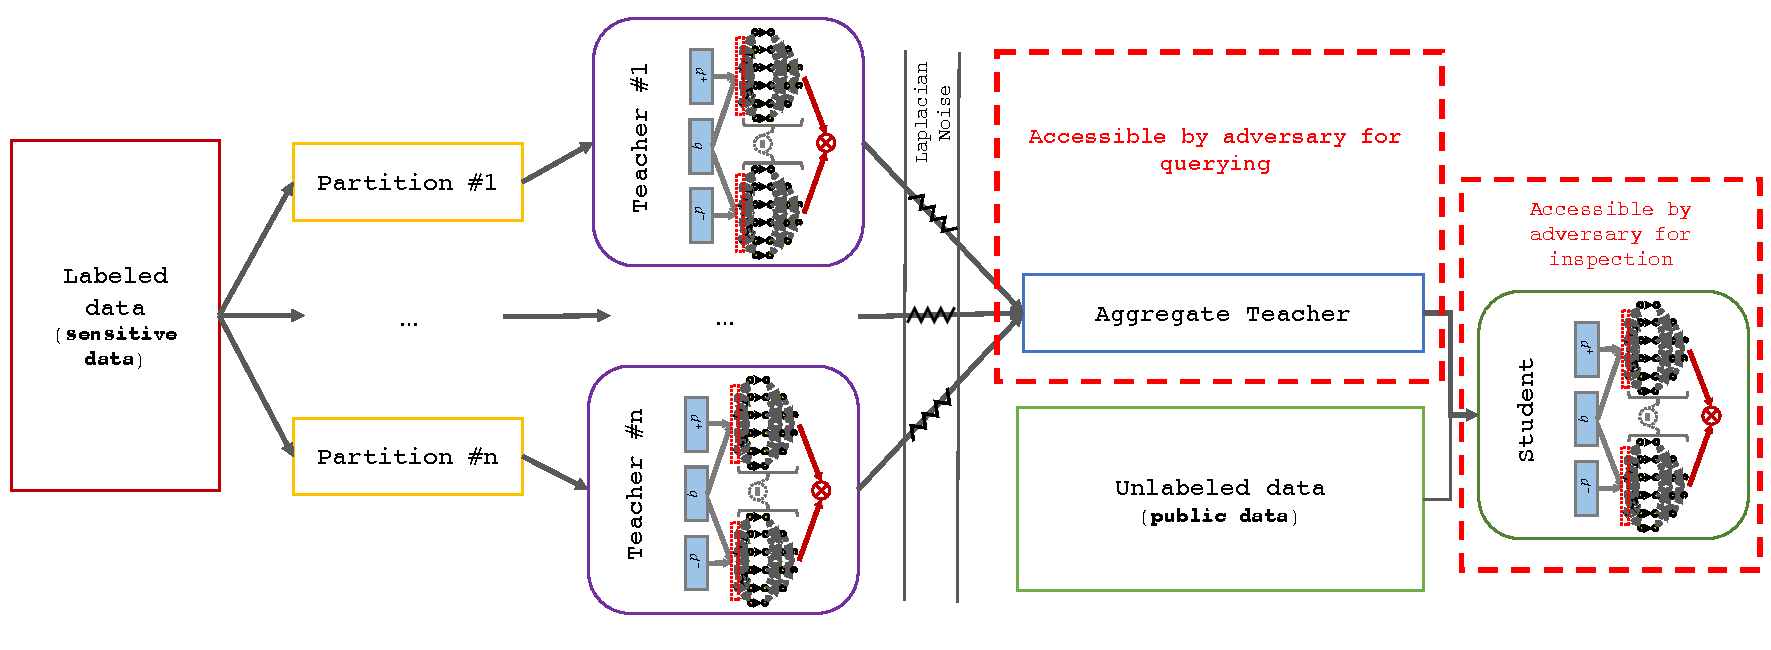
\includegraphics[height=5.5cm]{03-part-02/chapter-04/figs_and_tables/fig_privacy_preserving_ranker_model.pdf}%
    \caption{\label{fig:pp_model} Privacy preserving annotator/model sharing, proposed by~\citet{Papernot:2017}.}
\end{figure}

The general schema of the PATE is illustrated in Figure~\ref{fig:pp_model}. First, the sensitive training data is divided into $n$ partitions. Then, on each partition, an independent neural network model is trained as a teacher.  Once all the teachers are trained, an aggregation step is done using majority voting to generate a single global prediction.  
Laplacian noise is injected into the output of the prediction of each teacher before aggregation. The introduction of this noise is what protects privacy because it obfuscates the vulnerable cases, where teachers disagree. 

The aggregated teacher can be considered as a deferentially private API to which we can submit the input and it then returns the privacy preserving label. There are some circumstances where due to efficiency reasons the model is needed to be deployed to the user device~\cite{Abadi:2016}. To be able to generate a shareable model where the privacy of the training data is preserved, \citet{Papernot:2017} train an additional model called the student model. The student model has access to unlabeled public data during training. The unlabeled public data is annotated using the aggregated teacher to transfer knowledge from teachers to student model in a privacy preserving fashion. 
This way, if the adversary tries to recover the training data by inspecting the parameters of the student model, in the worst case, the public training instances with privacy preserving labels from the aggregated teacher are going to be revealed.  The privacy guarantee of this approach is formally proved using differential privacy framework.

As there is no publicly available large scaled data that we can use in our experiments as the initial sensitive labeled data, we use pseudo labels as it is explained in~\ref{sec:pseudo_labeling}\footnote{Partitioning the fully supervised training data in our problem leads to very small training sets which are not big enough to train teacher networks.}. 
In our experiments, we split the training data into three partitions, each contains one million queries annotated by the BM25 method. We train three identical teacher models. Then, we use the aggregated noisy predictions from these teachers to train the student network using the knowledge distillation approach. Configurations of teacher and student networks are similar to the previous experiments, as they are presented in Table~\ref{tbl:cfg}.

We evaluate the performance in two situations: In the first one, the privacy parameter, which determines the amount of noise, is set to zero, and in the second one, the noise parameter is set to $0.05$, which guarantees a low privacy risk~\citep{Papernot:2017}.
%
We report the average performance of the teachers before noise, the performance of noisy and non-noisy aggregated teacher, and the performance of the student networks in two situations.  The results of these experiments are reported in Table~\ref{tbl_res2}.

\begin{table}[t]
\centering
\caption{\label{tbl_res2}Performance of the teachers (average) and student models with noisy and non-noisy aggregation.}
\vspace{5pt}
\begin{adjustbox}{max width=\textwidth}
\begin{tabular}{l c c c}
\toprule
 \bf Model & \textbf{MAP} & \textbf{P@20} & \textbf{nDCG@20} 
\\ \midrule
{Teachers (avg)} 
& 0.2566 & 0.3300 & 0.3836
\\ \midrule
{Non-noisy aggregated teacher} 
& 0.2380 & 0.3055 & 0.3702 
\\
{Student \small{(non-noisy aggregation)}} 
& 0.2337 & 0.3192 & 0.3717
\\ \midrule 
{Noisy aggregated teacher} 
& 0.2110 & 0.2868 & 0.3407 
\\
{Student \small{(noisy aggregation)}} 
& 0.2255 & 0.2984 & 0.3559 
\\ \bottomrule
\end{tabular}
\end{adjustbox}
\end{table}

Results in Table~\ref{tbl_res2} suggest that using the noisy aggregation of multiple teachers as the supervision signal, we can train a neural ranker with an acceptable performance.
%
Compared to the single teacher setup in Section~\ref{sec:mimic_learning_to_rank}, the performance of the student network is not as good as the average performance of teachers. Although the student network performs better than the teacher in the noisy aggregation setup. This is more or less the case for a student together with a non-noisy aggregated teacher.
% 
We believe drops in the performance on the student networks compared to the results in Section~\ref{sec:mimic_learning_to_rank} are not just due to partitioning, noise, and aggregation. This is also the effect of the change in the amount of training data for the teachers in our experiments. We speculate that in the case of having enough training data in each partition for each teacher, their prediction will be more determined and we will have less disagreement in the aggregation phase and consequently, we will get better signals for training the student model.



\section{Related Work}
In this section, we briefly review the neural ranking models in terms of their general architectures and discuss how the neural models proposed in this chapter are related to the previous works.

Recently, several attempts have been made to study deep neural networks in IR applications, which can be generally partitioned into two categories~\citep{guo2019deep, Onal:2016, Zhang:2016}. 
The first category includes approaches that use the results of trained (deep) neural networks in order to improve the performance in IR applications. Among these, distributed word representations or embeddings~\citep{Mikolov:2013,Pennington:2014} have attracted a lot of attention. Word embedding vectors have been applied to term re-weighting in IR models~\citep{Zheng:2015}, query expansion~\citep{Diaz:2016,Zamani:2016a}, query classification~\citep{Liu:2015,Zamani:2016b},  etc. 
The main shortcoming of most of the approaches in this category is that the objective of the trained neural network differs from the objective of these tasks.  For instance, the word embedding vectors proposed in~\citep{Mikolov:2013,Pennington:2014} are trained based on term proximity in a large corpus, which is different from the objective in most IR tasks. \citet{Zamani:2017} recently proposed relevance-based word embedding models for learning word representations based on the objectives that matter for IR applications.

The second category, which the models proposed in this chapter belong to, consists of the approaches that design and train a (deep) neural network for a specific task, e.g., question answering~\citep{Cohen:2016,Yang:2016}, click models~\citep{Borisov:2016}.
A number of the approaches in this category have been proposed for ranking documents in response to a given query.
These approaches can be generally divided into two groups: \emph{late combination models} and \emph{early combination models} (or representation-focused and interaction-focused models according to~\citep{Guo:2016}). 
The late combination models, following the idea of Siamese networks~\citep{Bromley:1993}, independently learn a representation for each query and candidate document and then calculate the similarity between the two estimated representations via a similarity function. For example, \citet{Huang:2013} proposed DSSM, which is a feed forward neural network with a word hashing phase as the first layer to predict the click probability given a query string and a document title. 
The DSSM model was further improved by incorporating convolutional neural networks~\citep{Shen:2014}.

On the other hand, the early combination models are designed based on the interactions between the query and the candidate document as the input of network. 
For instance, DeepMatch~\citep{Lu:2013} maps each text to a sequence of terms and trains a feed-forward network for computing the matching score. 
The deep relevance matching model for ad-hoc retrieval~\citep{Guo:2016} is another example of an early combination model that feeds a neural network with the  histogram-based features representing interactions between the query and document. 
Early combining enables the model to have an opportunity to capture various interactions between query and document(s), while with late combination approach, the model has only the chance of isolated observation of input elements. Recently, Mitra et al.~\citep{Mitra:2016} proposed to simultaneously learn local and distributional representations, which are early and late combination models respectively,  to capture both exact term matching and semantic term matching.

Until now, all the proposed neural models for ranking are trained on either explicit relevance judgements or clickthrough logs. However, a massive amount of such training data is not always available. 

In this chapter, we propose to train neural ranking models using weak supervision, which is the most natural way to reuse the existing supervised learning models where the imperfect labels are treated as the ground truth.
The basic assumption is that we can cheaply obtain labels (that are of lower quality than human-provided labels) by expressing the prior knowledge we have about the task at hand by specifying a set of heuristics, adapting existing ground truth data for a different but related task (this is often referred to distant supervision\footnote{We do not distinguish between weak and distant supervision as the difference is subtle and both terms are often used interchangeably in the literature.}), extracting supervision signal from external knowledge-bases or ontologies, crowd-sourcing partial annotations that are cheaper to get, etc.
%
Weak supervision is a natural way to benefit from unsupervised data and it has been applied in NLP for various tasks including relation extraction~\citep{Bing:2015,Han:2016}, knowledge-base completion~\citep{Hoffmann:2011}, sentiment analysis~\citep{Severyn:2015:SemEval}, etc.  
There are also similar attempts in IR for automatically constructing test collections~\citep{Asadi:2011} and learning to rank using labeled features, i.e., features that an expert believes they are correlated with relevance~\citep{Diaz:2016:ictir}.
In this chapter, we make use of traditional IR models as the weak supervision signal to generate a large amount of training data and train effective neural ranking models that outperform the baseline methods by a significant margin.


%%%%%%%%%%%%%%%%%%%%%%%%%%%%%%%%%%%%%%%%%%%%%%%%%%%%%%%%%%%%%%%%%%%%%%%%%%%%%%%%%%%%%%%%%%%%%%%%%%%%%%%%%%%%%%%%%%%%%%%%%%%%%%%%%%%%%%%%%%%%%%%%%%%%%%%%%%%%%%%%%%%%%%%%%%%%%%%%%%%%%%%%%%%%%%%%%%%%%%%%%%%%%%%%%%%%%%%%%%%%%%%%%%%%%%%%%%%%%%%%%%%%%%%%%%%%%%%%%%%%%%%%%%%%%%%%%%%%%%%%%%%%%%%%%%%%%%%%%%%%%%%%%%%%%%%%%%%%%%%%%%%%%%%%%%



To circumvent the lack of human-labeled training examples, unsupervised learning methods aim to model the underlying data distribution, thus learning powerful feature representations of the input data, which can be helpful for building more accurate discriminative models especially when little or even no supervised data is available. A large group of unsupervised neural models seeks to exploit the implicit internal structure of the input data, which in turn requires customized formulation of the training objective (loss function), targeted network architectures and often non-trivial training setups. 


For example in NLP, various methods for learning distributed word representations, e.g., word2vec~\citep{Mikolov:2013}, GloVe~\citep{Pennington:2014}, and sentence representations, e.g., paragraph vectors~\citep{Le:2014} and skip-thought~\citep{Kiros:2015} have been shown very useful to pre-train word embeddings that are then used for other tasks such as sentence classification, sentiment analysis, etc. Other generative approaches such as language modeling in NLP, and, more recently, various flavors of auto-encoders~\citep{Baldi:2012} and generative adversarial networks~\citep{Goodfellow:2014} in computer vision have shown a promise in building more accurate models.






A lot of research has been done on the general problem of preserving the privacy of sensitive data in IR applications, where the question is how should we design effective IR systems without damaging users' privacy?  One of the solutions so far is to anonymize the data and try to hide the identity of users~\citep{Carpineto:2013, Zhang:2016}.  As an example, \citet{Zhang:2016} use a differential privacy approach for query log anonymization. However, there is no guarantee that the anonymized data will be as effective as the original data.

Modeling privacy in machine learning is a challenging problem and there has been much research in this area. Preserving the privacy of deep learning models is even more challenging, as there are more parameters to be safeguarded~\citep{Phan:2016}. 
Some work has studied the vulnerability of deep neural network as a service, where the interaction with the model is only via an input-output black box~\citep{Tramer:2016, Fredrikson:2015, Shokri:2016}.
Others have proposed approaches to protect privacy against an adversary with a full knowledge of the training mechanism and access to the model's parameters. For instance, \citet{Abadi:2016} propose a privacy preserving stochastic gradient descent algorithm offering a trade-off between utility and privacy. More recently, \citet{Papernot:2017} propose a semi-supervised method for transferring the knowledge for deep learning from private training data. They propose a setup for learning privacy-preserving student models by transferring knowledge from an ensemble of teachers trained on disjoint subsets of the data for which privacy guarantees are provided.


\section{Conclusion}
In this chapter, we proposed to use unsupervised methods in order to programmatically generate large amounts of training data, as weakly annotated data, to train effective neural ranking models.
We focus on the task of assessing relevance, i.e. ranking documents given a query that suffers from a large-scale publicly available training set
We examine various neural ranking models with different ranking architectures and objectives, and different input representations. 

We used over six million queries to train our models and evaluated them on Robust04 and ClueWeb 09-Category B collections, in an ad-hoc retrieval setting.  The experiments showed that our best performing model significantly outperforms the BM25 model (our weak supervision signal) by over $13\%$ and $35\%$ MAP improvements in the Robust04 and ClueWeb collections, respectively. 
We also demonstrated that in the case of having a small amount of training data, we can improve the performance of supervised learning by pre-training the network on weakly supervised data.

Based on our results, there are three key ingredients in neural ranking models that lead to good performance with weak supervision:
%
The first is the proper input representation. Providing the network with raw data and letting the network to learn the features that matter, gives the network a chance of learning how to ignore imperfection in the training data.
%
The second ingredient is to target the right goal and define a proper objective function. In the case of having weakly annotated training data, by targeting some explicit labels from the data, we may end up with a model that learned to express the data very well, but is incapable of going beyond it. 
This is especially the case with deep neural networks where there are many parameters and it is easy to learn a model that overfits the data.
%
The third ingredient is providing the network with a considerable amount of training examples. 
As an example, during the experiments we noticed that using the \feedthree, the network needs a lot of examples to learn embeddings that are more effective for retrieval compared to pre-trained embeddings. 
Thanks to weak supervision, we can generate as much training data as we need with almost no cost.


We also study how learning from weak signals can benefit preserving privacy where some noise is intentionally added to the training signal to preserve the privacy. We employed Private Aggregation of Teacher Ensembles (PATE)~\citep{Papernot:2017}  to train a privacy preserving neural ranking model, in which we train several neural rankers on disjoint subsets of the training data and use the noisy aggregated signals from these models on an unlabeled set to train a neural ranker that in a setup that guarantees a certain level of differential privacy.
These experiments lays the groundwork for the idea of sharing a privacy preserving model instead of sensitive data in IR applications. This suggests researchers from industry share the knowledge learned from actual users' data with the academic community that leads to a better collaboration of all researchers in the field. 